\documentclass[11pt,answers]{exam}

\usepackage{etex}
\usepackage{amssymb,amsmath,multicol} %<-- InWorksheetExam1 i also have fancyhdr,

\usepackage[metapost]{mfpic}
\usepackage[pdftex]{graphicx}
\usepackage{tabu}

\usepackage{pst-plot}
\usepackage{pgfplots}
\pgfplotsset{compat=1.9}

\usepackage{tikz}
\usepackage{tkz-2d}
\usepackage{tkz-base}
\usetikzlibrary{calc}
\usetikzlibrary{arrows}

\usepackage{systeme}

\usepackage[inline]{enumitem}
\usepackage{refcount}%<-- non in WorksheetExam1

\usepackage{pstricks-add,pst-eucl}
\usepackage{systeme}
\usepackage{setspace}
\usepackage{multicol}


\usepackage[inline]{enumitem}   
\makeatletter
% This command ignores the optional argument for itemize and enumerate lists
\newcommand{\inlineitem}[1][]{%
\ifnum\enit@type=\tw@
    {\descriptionlabel{#1}}
  \hspace{\labelsep}%
\else
  \ifnum\enit@type=\z@
       \refstepcounter{\@listctr}\fi
    \quad\@itemlabel\hspace{\labelsep}%
\fi}
\makeatother


\def\f{x+1} \def\g{-x/3+2}  \def\h{-x+3}

\newcommand{\vasymptote}[2][]{
    \draw [densely dashed,#1] ({rel axis cs:0,0} -| {axis cs:#2,0}) -- ({rel axis cs:0,1} -| {axis cs:#2,0});
}

\boxedpoints

\addpoints
%\printanswers
\noprintanswers

\opengraphsfile{Q12a_Fa18}

\begin{document}
\extrawidth{-0.3in}
\pagestyle{headandfoot}

\setlength{\hoffset}{-.25in}

\extraheadheight{-.3in}
\runningheadrule
\firstpageheader{\bfseries {Precalculus}}{ \bfseries {Quiz 12 }}{\bfseries {12/11/18}} 

\begin{center}
	This quiz has \numquestions\ questions, for a total of \numpoints\
	points and \numbonuspoints\ bonus points.
\end{center}


\firstpagefooter{} %%&&CHANGED
                {}
                {%Points earned: \hbox to 0.5in{\hrulefill}
                % out of  \pointsonpage{\thepage} points
                }
                 
						

\vspace*{0.1cm}
\hbox to \textwidth { \scshape {Name:} \enspace\hrulefill}
\vspace{0.1cm}




\pointpoints{point}{points}

\begin{questions}


\addpoints


 \question[2] Write the exact values of the two solutions of the equation $\displaystyle \sin x = 0.4$ in $[0,2\pi]$.
  
 	
 	\fillwithdottedlines{1.1in}
 	\bigskip
 
\question[2] The chance of a significant cloud cover in a city on day $t$ of the year (with January 1st corresponding to $t=0$) is given by the formula $\displaystyle D(t)=20\cos \left ( \frac{2\pi}{360}(t-1)\right )+50$. Note that $D$ is already written as a percent, so for example the chance of a significant cloud cover on January 2nd is $D(0)=70\%$. Find the exact values of $t$ ($0\leq t \leq 365$) when the model predicts that the chance of a significant cloud cover is 50\%. 

 	\fillwithdottedlines{1.3in}
 	\bigskip
 \question[2] A certain bay with very high tides displays the following behavior. In one 12-h period the water starts at mean sea level, rises to 11.5 ft above, drops to 11.5 ft below, then returns to mean sea level. Let $y$ be the height above sea level in feet, and $t$ the number of hours since the start of the 12-h period.	 Assuming that the motion of the tides is simple harmonic (so the equation for $y$can be represented as a sinusoidal function of the form $y=a\sin(Bt)$ or $y=a\cos Bt)$, find an equation that describes the height of the tide in this bay above mean sea level. 
 
  	\fillwithdottedlines{1.3in}
  	\bigskip
  	
  	\question[1] Find the exact value of $\displaystyle \sin^{-1}\left ( -\frac{\sqrt{2}}{2} \right )$. \dotfill
  	\bigskip
  	
 \bonusquestion[1] True or false?
 $\displaystyle \sin^{-1}\left ( \sin \left ( \frac{4\pi}{3}\right ) \right ) = \frac{4\pi}{3}$.
 \begin{oneparchoices}
 	\choice True \choice False
 	\end{oneparchoices}
\end{questions}
\newpage

\par\medskip\hrule\medskip


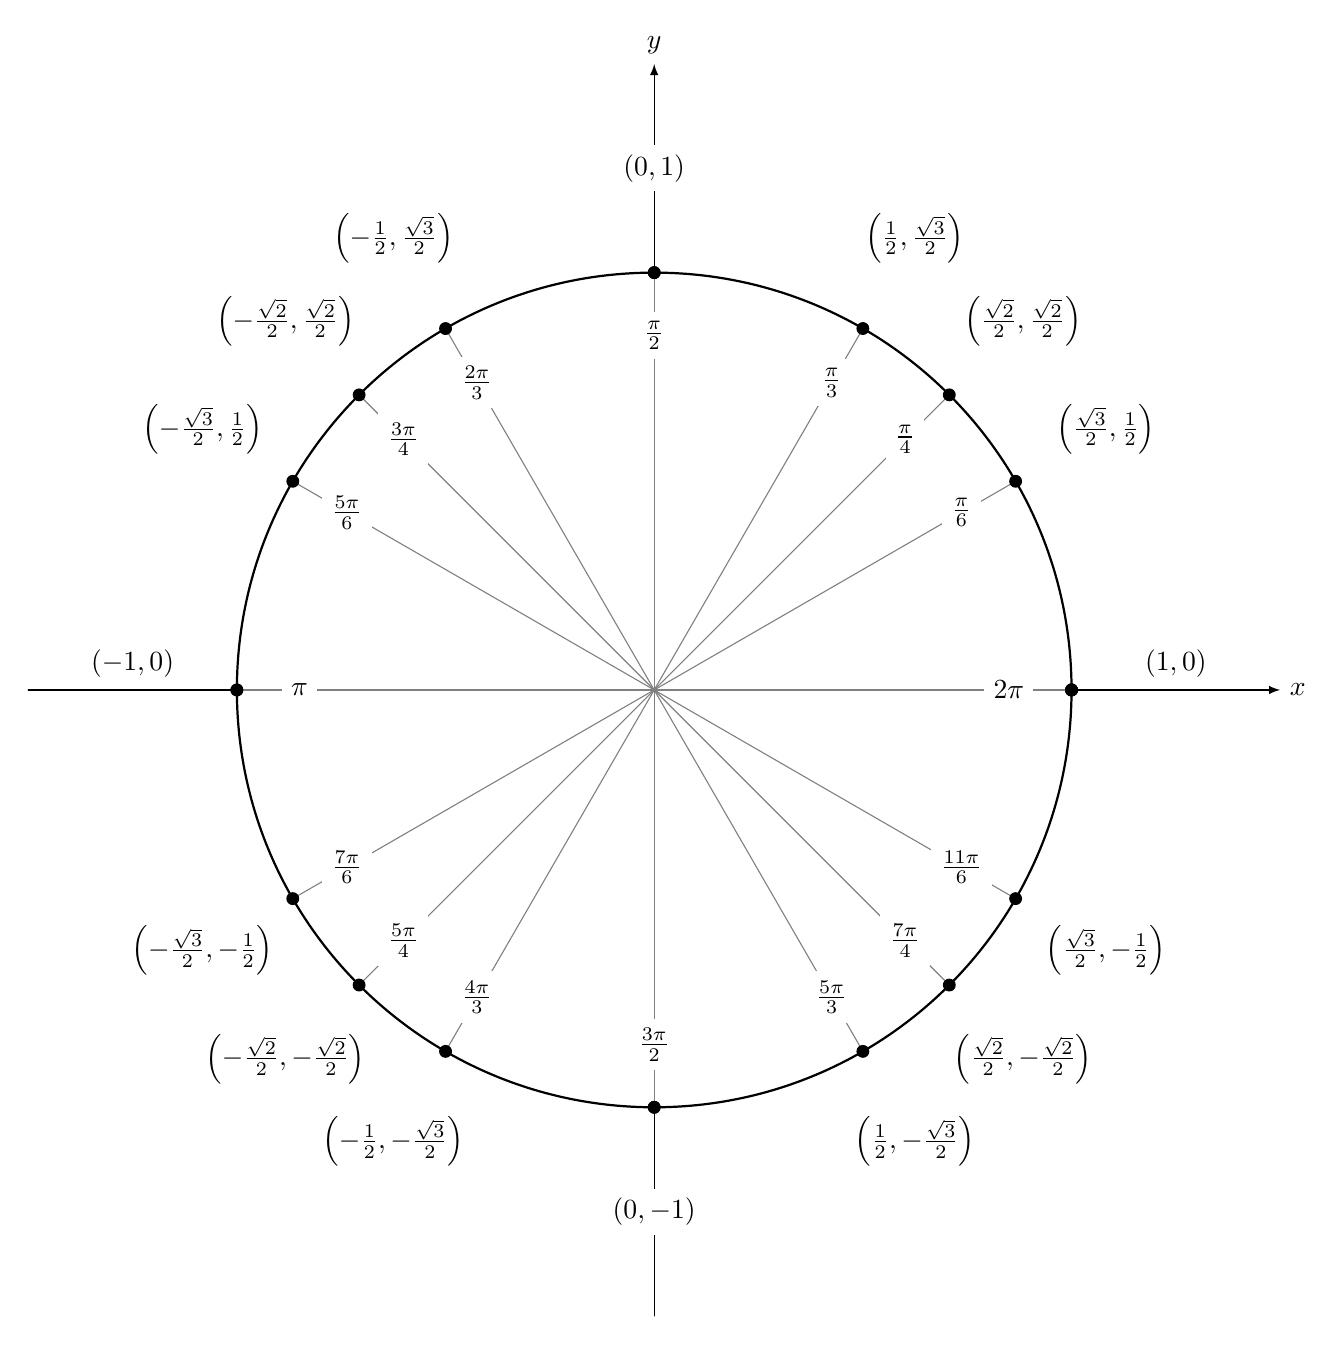
\begin{tikzpicture}[scale=5.3,cap=round,>=latex]
% draw the coordinates
\draw[->] (-1.5cm,0cm) -- (1.5cm,0cm) node[right,fill=white] {$x$};
\draw[->] (0cm,-1.5cm) -- (0cm,1.5cm) node[above,fill=white] {$y$};

% draw the unit circle
\draw[thick] (0cm,0cm) circle(1cm);

\foreach \x in {0,30,...,360} {
	% lines from center to point
	\draw[gray] (0cm,0cm) -- (\x:1cm);
	% dots at each point
	\filldraw[black] (\x:1cm) circle(0.4pt);
	% draw each angle in degrees
	%\draw (\x:0.6cm) node[fill=white] {$\x^\circ$};
}

\foreach \x in {0,45,...,360} {
	% lines from center to point
	\draw[gray] (0cm,0cm) -- (\x:1cm);
	% dots at each point
	\filldraw[black] (\x:1cm) circle(0.4pt);
	% draw each angle in degrees
	%\draw (\x:0.6cm) node[fill=white] {$\x^\circ$};
}
% draw each angle in radians
\foreach \x/\xtext in {
	30/\frac{\pi}{6},
	45/\frac{\pi}{4},
	60/\frac{\pi}{3},
	90/\frac{\pi}{2},
	120/\frac{2\pi}{3},
	135/\frac{3\pi}{4},
	150/\frac{5\pi}{6},
	180/\pi,
	210/\frac{7\pi}{6},
	225/\frac{5\pi}{4},
	240/\frac{4\pi}{3},
	270/\frac{3\pi}{2},
	300/\frac{5\pi}{3},
	315/\frac{7\pi}{4},
	330/\frac{11\pi}{6},
	360/2\pi}
\draw (\x:0.85cm) node[fill=white] {$\xtext$};

\foreach \x/\xtext/\y in {
	% the coordinates for the first quadrant
	30/\frac{\sqrt{3}}{2}/\frac{1}{2},
	45/\frac{\sqrt{2}}{2}/\frac{\sqrt{2}}{2},
	60/\frac{1}{2}/\frac{\sqrt{3}}{2},
	% the coordinates for the second quadrant
	150/-\frac{\sqrt{3}}{2}/\frac{1}{2},
	135/-\frac{\sqrt{2}}{2}/\frac{\sqrt{2}}{2},
	120/-\frac{1}{2}/\frac{\sqrt{3}}{2},
	% the coordinates for the third quadrant
	210/-\frac{\sqrt{3}}{2}/-\frac{1}{2},
	225/-\frac{\sqrt{2}}{2}/-\frac{\sqrt{2}}{2},
	240/-\frac{1}{2}/-\frac{\sqrt{3}}{2},
	% the coordinates for the fourth quadrant
	330/\frac{\sqrt{3}}{2}/-\frac{1}{2},
	315/\frac{\sqrt{2}}{2}/-\frac{\sqrt{2}}{2},
	300/\frac{1}{2}/-\frac{\sqrt{3}}{2}}
\draw (\x:1.25cm) node[fill=white] {$\left(\xtext,\y\right)$};

% draw the horizontal and vertical coordinates
% the placement is better this way
\draw (-1.25cm,0cm) node[above=1pt] {$(-1,0)$}
(1.25cm,0cm)  node[above=1pt] {$(1,0)$}
(0cm,-1.25cm) node[fill=white] {$(0,-1)$}
(0cm,1.25cm)  node[fill=white] {$(0,1)$};
\end{tikzpicture}



\end{document}                 